
%----------------------------------------------------------------------------------------
%	PACKAGES AND THEMES
%----------------------------------------------------------------------------------------

\documentclass{beamer}
\mode<presentation> {
\usetheme{Berlin}
}
\AtBeginSection[]{
  \begin{frame}
  \vfill
  \centering
  \begin{beamercolorbox}[sep=8pt,center,shadow=true,rounded=true]{title}
    \usebeamerfont{title}\insertsectionhead\par%
  \end{beamercolorbox}
  \vfill
  \end{frame}
}
\usepackage{graphicx} % Allows including images
\usepackage{booktabs} % Allows the use of \toprule, \midrule and \bottomrule in tables

%----------------------------------------------------------------------------------------
%	TITLE PAGE
%----------------------------------------------------------------------------------------
\titlegraphic{
\includegraphics[width=5.5cm]{photo/ohm_logo.png}}

\title[Department of Computer Science]{IT-based Automatic Text Summarization with the Use of Textgeneration Methods} % The short title appears at the bottom of every slide, the full title is only on the title page
\author{L\"ohr Tim} 
\institute[Prof. Dr. Alfred Holl] % Your institution as it will appear on the bottom of every slide, may be shorthand to save space
{
Technische Hochschule Nürnberg Georg Simon OHM\\ % Your institution for the title page
\medskip
\textit{Bachelor Thesis | Business Information Systems and Management} 
}
\date{\today} % Date, can be changed to a custom date
%----------------------------------------------------------------------------------------
\begin{document}

\begin{frame}
\titlepage % Print the title page as the first slide
\end{frame}
%----------------------------------------------------------------------------------------
\begin{frame}
\frametitle{Overview} % Table of contents slide, comment this block out to remove it
\tableofcontents % Throughout your presentation, if you choose to use \section{} and \subsection{} commands, these will automatically be printed on this slide as an overview of your presentation
\end{frame}
%
%----------------------------------------------------------------------------------------
%	PRESENTATION SLIDES
%----------------------------------------------------------------------------------------

%------------------------------------------------
\section{Introduction}

%------------------------------------------------

\begin{frame}
\frametitle{Clarify the Keywords}
Noticeably almost annually Artificial Intelligence is finding more and more its way into businesses. 
\begin{columns}
	\column{0.3\textwidth}
	\begin{figure}
		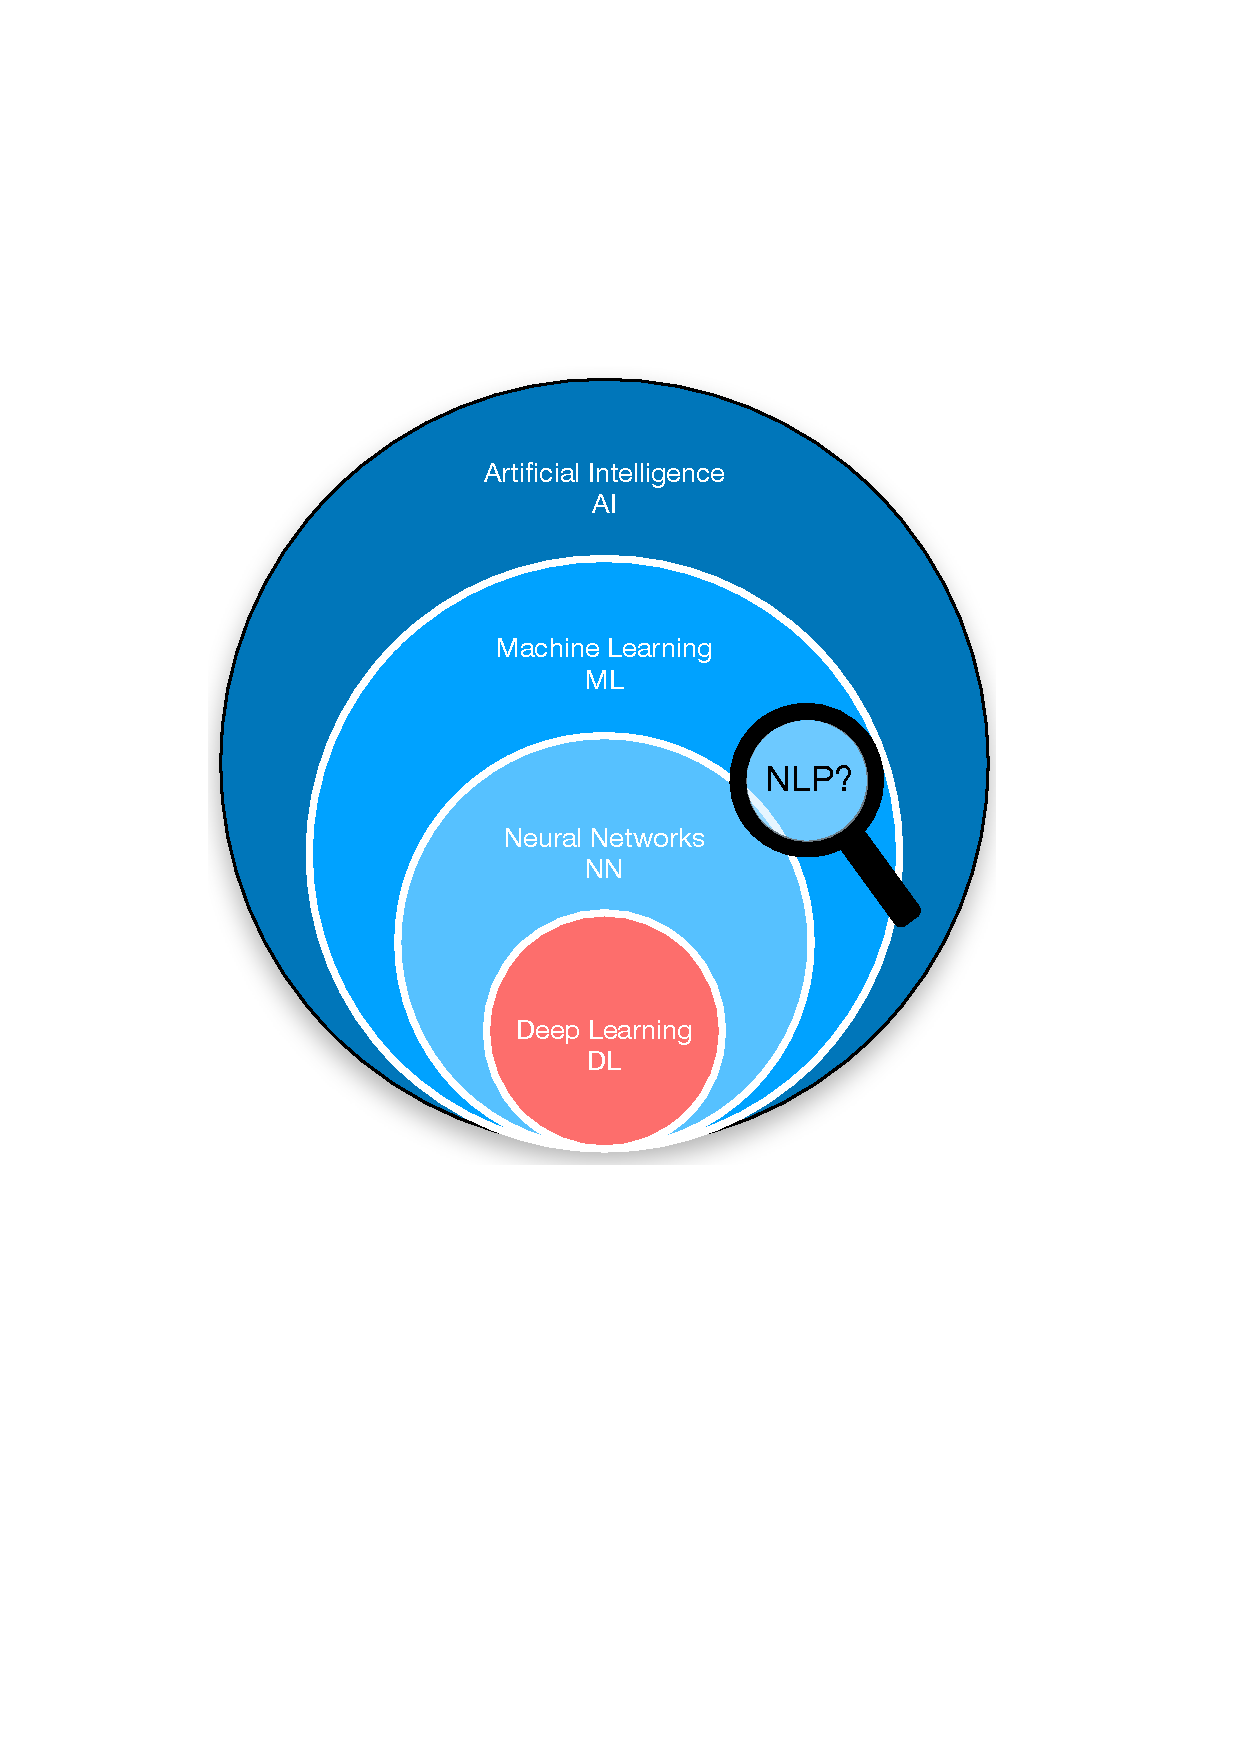
\includegraphics[width=1.15\linewidth]{photo/intro_0}
	\end{figure}
	\column{0.6\textwidth}
	\begin{block}{Famous phrases for Advertisement}
		\begin{enumerate}
			\item \textit{Our product is powered now by AI!} 
			\item \textit{We now use Deep Learning for a better performance!}
		\end{enumerate}
	\end{block}
\textbf{In conclusion:} Deep Learning is a technique making use of Neural networks. Those are methods of Machine Learning, which is itself just an application of the entire AI ecosystem.
\end{columns}
\end{frame}

%------------------------------------------------

\begin{frame}
\frametitle{Classify my Thesis in this Ecosystem}
\begin{block}{NLP}
	Natural Language Processing (NLP) deals and manipulates data in form of our language to gain new information from it or perform other related tasks such as Text Summarization.
\end{block}

\begin{center}
	\textbf{Where is NLP located?} \\
\end{center}

Depending on what is performed, Natural Language Processing is either just an ML application, or like in my case, it can even make use of Neural Networks with Deep Learning methods to generate better results!

\end{frame}

%------------------------------------------------
\section{State of the Art}
%---------------------------------------------
\begin{frame}
\frametitle{General Methology}
Using data analysis and show how it can be used to improve the marketing of Airbnb in Seattle according to each policy of the marketing-mix.
\end{frame}
%
%------------------------------------------------
%
\begin{frame}
\frametitle{Marketing}
\begin{columns}[c] % The "c" option specifies centered vertical alignment while the "t" option is used for top vertical alignment

\column{.45\textwidth} % Left column and width
\textbf{The 4 P's of the Marketing-Mix}
\begin{enumerate}
\item Product
\item Price
\item Promotion
\item Place
\end{enumerate}

\column{.5\textwidth} % Right column and width

\begin{block}{Definition Marketing}
Marketing is about the firm’s effort to address customer needs and expectations, which influences the demands made by the customers on the product and need to be fulfilled by the product.
\end{block}
\end{columns}
\end{frame}

%------------------------------------------------

\begin{frame}
\frametitle{How to use Data Analysis to improve the Airbnb Marketing?}
\begin{itemize}
\item \textbf{Descriptive analysis:} Reviews, locations, review and price correlation, details of listings and price correlation
\item \textbf{Descriptive analysis:} Predict the number of customer
\item \textbf{Optimization:} Optimize the booking of listings 
\item \textbf{Adaptive learning:} Learn from the results generated and combine results to give out suggestion in marketing campaigns may hold by Airbnb
\end{itemize}
\end{frame}

%------------------------------------------------

\begin{frame}
	\frametitle{Reviews comparison}
	We can see a correlation between the amount of reviews and the accommodation counts. 
	\begin{figure}
		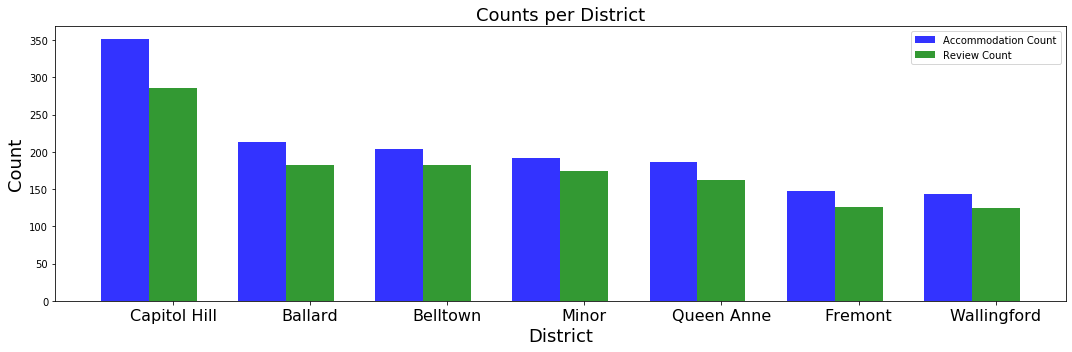
\includegraphics[width=0.8\linewidth]{photo/3_count_per_district}
	\end{figure}
\end{frame}

%------------------------------------------------

\begin{frame}
	\frametitle{Linear Regression}
	\begin{columns}[c] % The "c" option specifies centered vertical alignment while the "t" option is used for top vertical alignment
		
		\column{.45\textwidth} % Left column and width
		\begin{itemize}
			\item Use a Linear function and estimate its parameters
			\item There are different approaches to estimate the parameters
			\item The accuracy of a model can be compared with different loss functions
		\end{itemize}
		
		\column{.45\textwidth} % Right column and width
		The fitted line can mathematically described as:
		\begin{equation}
		Y_i = \beta_0 + \beta_1 X_i + \epsilon_i
		\end{equation}
		
	\end{columns}
\end{frame}

%------------------------------------------------

\section{Prototype}
%--------------------------------------------

\begin{frame}
\frametitle{Multinomial Naive Bayes}
\begin{columns}[c] % The "c" option specifies centered vertical alignment while the "t" option is used for top vertical alignment

\column{.45\textwidth} % Left column and width
\begin{itemize}
\item Assumes conditionally independent classes
\item Probability of observing features \(f_1\)  \\
through \(f_n\) , given some class \(c\)
\end{itemize}

\column{.45\textwidth} % Right column and width
\begin{equation}
p(f_1,..., f_n|c) = \prod_{i=1}^n p(f_i|c)
\end{equation}
This means that when I want to use a Naive Bayes model to classify a new example, the posterior probability is much simpler to work with:
\begin{equation}
p(c|f_1,...,f_n) \propto p(c)p(f_1|c)...p(f_n|c)
\end{equation}
\end{columns}
\end{frame}

%------------------------------------------------
\begin{frame}
\frametitle{LSTM Neural Network}
\begin{itemize}
\item Long Short Term Memory Neural Network is based on the Recurrent Neural Network
\item It is very well suited for timeseries analysis like the prediction of price
\item Futher explanation exceeds this presentation
\end{itemize}
\begin{figure}
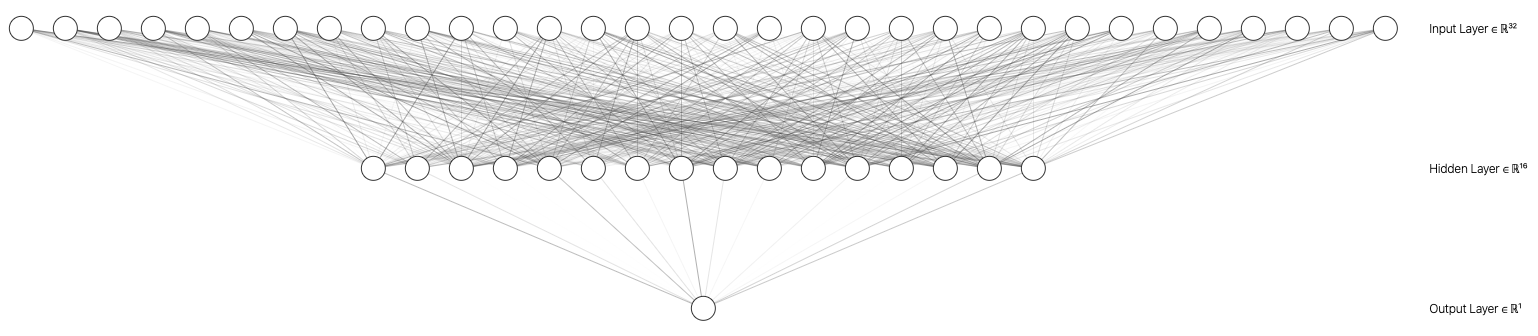
\includegraphics[width=0.8\linewidth]{photo/nn}
\end{figure}
\end{frame}

%------------------------------------------------
\section{Evaluation}
%--------------------------------------------
\begin{frame}
The team around Josh Keating reached a mean absolute error between 32\$ to 35\$
\begin{itemize}
\item Our network design was way to simple
\item We didn't include the important neighbourhood feature
\item Our result with our LSTM neural network was 64.04\$ (MSA)
\item Nevertheless, our best model was the linear regression with a MAE of 43.89\$
\end{itemize}
\end{frame}

%------------------------------------------------

\end{document} 